\begin{frame}
    \frametitle{Sistemas de numeraci\'on}
    \begin{itemize}
        \item La aritm\'etica es una \emph{herramienta}\pause
        \item ?`Una herramienta pr\'actica?:
            \begin{itemize}
                \item ?`Un \'unico s\'imbolo s\'imbolo? \pause
                \item ?`Un s\'imbolo por cada caso? \pause
            \end{itemize}
    \end{itemize}
    \textcolor{red}{Un conjunto reducido de s\'imbolos y reglas de combinaci\'on}
    \begin{itemize}
        \item Hexadecimal: 16 s\'imbolos (0 - 9 y A-F)
        \item Octal: 8 s\'imbolos (0 - 7)
        \item Binario: 2 s\'imbolos(0 y 1)
    \end{itemize}
\end{frame}
\note{
    \begin{enumerate}
        \item A tool to represent the world. to show us what we see.
        \item Examples about gazelles. One, two, many?
        \item Using pebbles? It must be practical, otherwise what is it good for
    \end{enumerate}
    \begin{itemize}
        \item We represent numbers with an underscore and teh base. 
        \item We assume all numbers are base 10.
    \end{itemize}
}

\begin{frame}
    \frametitle{Construyendo n\'umeros}
    \begin{block}{El n\'umero $1024_{10}$}
        $1024 = 1*10^3 + \pause 0*10^2 + \pause 2*10^1 +  4*10^0 $
    \end{block}
\end{frame}


\begin{frame}
    \frametitle{Los sistemas son equivalentes}
    \begin{block}{De base $n$ a base 10}
        $a = a_{n}*b^n + a_{n-1}*b^{n-1} + \ldots + a_{0} * b^{0}$
    \end{block}
    \pause
    \begin{block}{De base 10 a base $n$}
        \begin{itemize}
            \item Dividir el n\'umero por $n$ (divisi\'on entera). Registrar el Resto en Hexadecimal.
            \item Repetir con el cociente hasta que sea $0$.
        \end{itemize}
    \end{block}
\end{frame}

\begin{frame}
    \begin{ejercicio}{}
        Convertir $937_{10}$ a:
        \begin{itemize}
            \item Binario
            \item Ternario
            \item Cuaternario
            \item Octal
            \item Hexadecimal
        \end{itemize}
    \end{ejercicio}
    \pause
    \begin{ejercicio}{}
        Convertir $5ADC_{16}$ a: (hay un truco)
        \begin{itemize}
            \item Decimal
            \item Binario
            \item Ternario
            \item Cuaternario
            \item Octal
        \end{itemize}
    \end{ejercicio}
\end{frame}


\begin{frame}
    \begin{ejercicio}{}
        Responder:
        \begin{enumerate}
            \item Con 8 d\'igitos binarios (\emph{i.e.} un byte):  ?`cual es el mayor n\'umero que puedo representar en decimal?
            \item ?`Cu\'antos valores decimales distintos puedo generar con un byte?
        \end{enumerate}
    \end{ejercicio}

    \pause
    \begin{enumerate}
        \item $2^n - 1$
        \item $2^n$
    \end{enumerate}

\end{frame}

\subsection{Nuestro operador de archivos}

\begin{frame}
    \frametitle{Nuestro operario que no sabe leer $\ldots$}
    \pause
    \begin{itemize}
        \item Puede mirar: Prendido/Apagado, Hay/NoHay, 1/0, $\ldots$ \\
        \item Cuantos numeros puedo representar con binario.
    \end{itemize}
\end{frame}


\note{
    \begin{itemize}
        \item So the guy cannot read. What does he do? He needs to be able to understand that 10 is bigger than 9, but he cannot read!
        \item But he can ``feel''. He can feel power comming and not comming. Can't I then not combine it?
        \item What about the water? Make the example for the water circuit.
    \end{itemize}
}

\begin{frame}
    \frametitle{L\'ogica binaria}
    \begin{itemize}
        \item En base a 4 operaciones l\'ogicas: and, or, not, xor
    \end{itemize}
\end{frame}

\note{
    \begin{itemize}
        \item At this point I will draw the truth tables on teh board.
        \item Show the different circuits that can implement the logic. Explain that a combination of these is necessary.
    \end{itemize}
}

\subsection{Representaci\'on de la informaci\'on}

\begin{frame}
    \begin{itemize}
        \item ?`C\'omo se comunica que hay un nuevo papa? \pause
        \item ?`C\'omo funcionan los sem\'aforos? \pause
    \end{itemize}
    Un vocabulario basado en un alfabeto reducido.
\end{frame} 


\begin{frame}
    \frametitle{Codificando la informaci\'on}
    \begin{itemize}
        \item ?`Qu\'e necesitamos? \pause \textcolor{red}{Un convenio} 
        \item Hay varios: ASCII ( American Standard Code for Information Interchange ), UNICODE, UTF-8, $ldots$
    \end{itemize}

    \begin{table}[]
    \centering
    \begin{tabular}{lll}
        Decimal & Binario  & Char \\
        0       & 00000000 & NULL \\
        1       & 00000001 & SOH  \\
        2       & 00000010 & STX  \\
        ...     &          &      \\
        127     & 11111111 & DEL 
    \end{tabular}
    \end{table}
\end{frame}

\note{
    \begin{itemize}
        \item Explain that we need to represnet data in various ways.
        \item ASCII is one of them. ASCII is based on teletype: a typewriter that sent stuff via a cable.Think WW2 technology.
            \begin{itemize}
                \item It does not include any formatting information, but rather plaintext only
                \item Also, it includes some control characters.
            \end{itemize}
        \item What could the problems be? What happens with spanish? Could we use spanish?
    \end{itemize}
}

\begin{frame}
    \frametitle{Texto codificado en ASCII}
    \begin{block}{Universidad Paraguayo Alemana}
        01010101 01101110 01101001 01110110 01100101 01110010 01110011 01101001 01100100 01100001 01100100 00100000 01010000 01100001 01110010 01100001 01100111 01110101 01100001 01111001 01101111 00100000 01000001 01101100 01100101 01101101 01100001 01101110 01100001 
    \end{block}
\end{frame}

\begin{frame}
    \begin{ejercicio}{}
    Decodificar la siguiente secuencia ASCII: \\
        01100101 01101110 00100000 01110011 01101001 01101100 01100101 01101110 01100011 01101001 01101111 00100000 01110011 01100001 01101100 01101001 01110010 00100000 01100001 01101100 00100000 01110010 01100101 01100011 01110010 01100101 01101111
    \end{ejercicio}
\end{frame}

\note{
    Print and copy an ascii table for the people.
}

\subsection{Aritm\'etica en binario}

\begin{frame}
    \frametitle{Suma}
    \begin{table}[]
    \centering
    \begin{tabular}{lll}
        A & B & + \\
        0 & 0 & 0\\
        0 & 1 & 1\\
        1 & 0 & 1\\
        1 & 1 & 10 \\
    \end{tabular}
    \end{table}

    Ejemplo:
    $1010_{2} + 11_{2} = 1101_{2}$
\end{frame}

\begin{frame}
    \frametitle{Resta}
    La resta es m\'as compleja. Hay dos m\'etodos
    \begin{table}[]
    \centering
    \begin{tabular}{lll}
        A & B & - \\
        1 & 1 & 0\\
        0 & 0 & 0\\
        1 & 0 & 1\\
        0 & 1 & 0 (habiendo acarreado de la siguiente posici\'on)\\
    \end{tabular}
    \end{table}
    Ejemplo:
    $1010_{2} - 11_{2} = 0111_{2}$
\end{frame}

\begin{frame}
    \frametitle{Resta 1}
    $1010_{2} - 11_{2} = 0111_{2}$
    \begin{itemize}
        \item $0 - 1 = 1$ 
        \item $0 - 1 = 1$ \pause
        \item $1 - 0 = 1$ \pause
        \item $0 - 0 = 1$ \pause
    \end{itemize}
\end{frame}

\note{
    \begin{itemize}
        \item No fue posible hacer 0 -1, entonces acarreamos del anterior. Vienen dos por la posicion.
        \item No podemos acarrear del cero, asique tenemosq ue ir hasta qeu podamos y volver.
    \end{itemize}
}


\begin{frame}
    \frametitle{Resta 2}
    \begin{enumerate}
        \item Completar la cantidad de digitos para igualar los n\'umeros con ceros. \emph{e.g.} 01010 - 011 $\rightarrow$ 01010 - 00011
        \item Sumar el complemento
        \item Si la \'ultima sma tiene excedente, sumar ese excedente al resultado.
   \end{enumerate}
   \pause
    $1010_{2} - 11_{2} = 1010_{2} + 1100_{2} = (1)0110_{2} = 0110_{2} + 1_{2} = 0111_{2}$
\end{frame}

\begin{frame}
    \begin{ejercicio}{}
    Sumar:
        \begin{enumerate}
            \item 11 + 1	
            \item 11 + 11	
            \item 111 + 11	
            \item 111 + 10	
            \item 1110 + 111	
            \item 1100 + 110	
            \item 1111 + 10101	
            \item 1100 + 11001	
            \item 1011 + 1101	
            \item 1110 + 10111	
            \item 1110 + 1111	
            \item 11111 + 11101	
        \end{enumerate}
    \end{ejercicio}
\end{frame}

\begin{frame}
    \begin{ejercicio}{}
        Restar:
        \begin{enumerate}
            \item 11 - 10	
            \item 110 - 10	
            \item 1111 - 110	
            \item 100 - 10	
            \item 100 - 11	
            \item 1000 - 11	
            \item 1101 - 110	
            \item 11011 - 110	
            \item 1111 - 111	
            \item 110101 - 1010	
            \item 11011 - 111	
            \item 11110 - 111
        \end{enumerate}
    \end{ejercicio}
\end{frame}

\begin{frame}
    \frametitle{Multiplicaci\'on}
    \begin{enumerate}
        \item Copiar el primer factor cuando multiplicado por 1. Sino, una fila de 0
        \item Desplazar una columna a la izquierda al mover al siguiente digito del segundo factor. Repetir.
        \item Sumar todos los valores.
    \end{enumerate}
\end{frame}

\note{
    Make example of multiplication
}

\begin{frame}
    \begin{ejercicio}{}
        Multiplicar
        \begin{enumerate}
            \item 11 * 1	
            \item 11 * 11	
            \item 111 * 11	
            \item 111 * 10	
            \item 1110 * 111	
            \item 1100 * 110	
            \item 1111 * 10101	
            \item 1100 * 11001	
            \item 1011 * 1101	
            \item 1110 * 10111	
            \item 1110 * 1111	
            \item 11111 * 11101	
        \end{enumerate}
    \end{ejercicio}
\end{frame}


\begin{frame}
    \frametitle{Uniendo los cabos}
    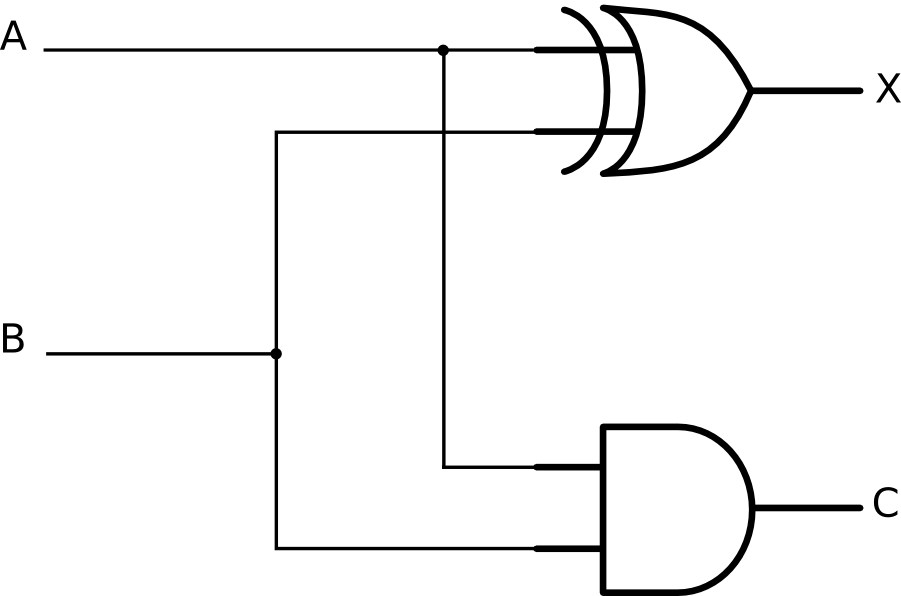
\includegraphics[scale=0.25]{./images/adder.png}
    \\
    \vspace{10mm}
    \begin{center}
        \huge{\textcolor{red}{?}}
    \end{center}

\end{frame}

\begin{frame}
    \frametitle{Uniendo los cabos}
    \begin{columns}
        \begin{column}{0.5\textwidth}
            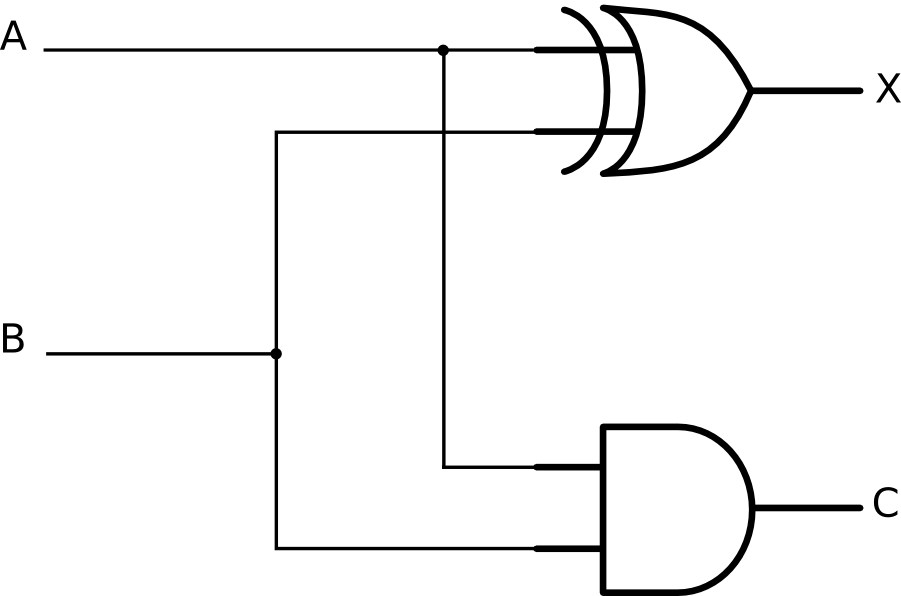
\includegraphics[scale=0.15]{./images/adder.png}
        \end{column}
        \begin{column}{0.5\textwidth}
                \begin{table}[]
                \centering
                \begin{tabular}{llll}
                    A & B & x & C\\
                    0 & 0 & 0 & 0\\
                    0 & 1 & 1 & 0\\
                    1 & 0 & 1 & 0\\
                    1 & 1 & 0 & 1\\
                \end{tabular}
                \end{table}
        \end{column}
    \end{columns}
\end{frame}

\note{
    \begin{itemize}
        \item Hablamos de representar la informaci\'on utilizando notaci\'on binaria y las cuatro operaciones.
        \item Mencionamos una cantidad de operaciones. Pero como funciona esto en binario y usando 4 operaciones?
        \item A dise\~nar un circuito
        \item Maybe remove this?
    \end{itemize}
}

\subsection{Fundamentos matem\'aticos de la computaci\'on}

\begin{frame}
    \frametitle{Los algoritmos}
    \begin{block}{Informalmente}
        Una colecci\'on de instrucciones para realizar una tarea espec\'ifica.
    \end{block}
    \pause
    \begin{block}{Formalmente}
        Secuencia de operaciones que puede ser interpretada por un sistema Turing-completo.
    \end{block}
\end{frame}

\note{
    \begin{itemize}
        \item Example about showering.
    \end{itemize}
}

\begin{frame}
    \frametitle{Las capacidades fundamentales de los sistemas de computaci\'on}
    \begin{itemize}
        \item Aut\'omatas 
        \item Complejidad \pause
        \item Computabilidad \pause
    \end{itemize}
    o\\
    ?`Qu\'e podemos calcular?
\end{frame}

\note{
    Introduce the concept of algorithm. That is, a procedure that needs to be done following a specific set of 
    steps. Some might be interchanged, some may not
}

\begin{frame}
    \frametitle{Aut\'omatas}
    Modelos computacionales
    \begin{itemize}
        \item Abstraer del dispositivo de c\'omputo (?`La ALU?) \pause
        \item ?`El poder del modelo?
    \end{itemize}
\end{frame}

\note{
    \begin{itemize}
        \item We are trying to reason on the computer, without getting lost in the complexities of the machine.
        \item But, not all models are good models. Gravity and high speeds, for example. We cannot use newtonian mechanics
            to explain quantum effects.
        \item We'll analyse the one model: FA.
    \end{itemize}
}


\begin{frame}
    \frametitle{Aut\'omatas de estado finito}
    Modelemos una puerta autom\'atica.
\end{frame}

\note{
    \begin{itemize}
        \item What do we need? That is, which elements to we need: Sensor, Door, Motor and the controller for the motor.
        \item If we wish to abstract, what do we care about? The door opening when someone comes, and closing when they leave.
    \end{itemize}
}


\begin{frame}
    \frametitle{El FA como reconocedor de lenguajes}
    \begin{center}
        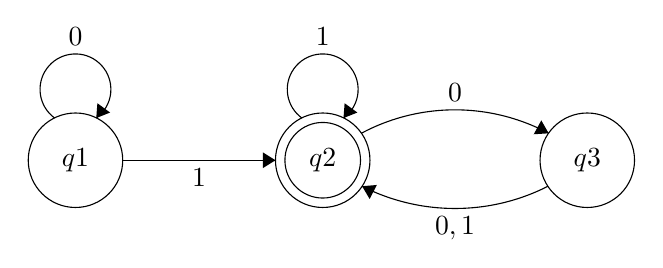
\begin{tikzpicture}[scale=0.2]
        \tikzstyle{every node}+=[inner sep=0pt]
        \draw [black] (16.4,-28.4) circle (3);
        \draw (16.4,-28.4) node {$q1$};
        \draw [black] (32.1,-28.4) circle (3);
        \draw (32.1,-28.4) node {$q2$};
        \draw [black] (32.1,-28.4) circle (2.4);
        \draw [black] (48.9,-28.4) circle (3);
        \draw (48.9,-28.4) node {$q3$};
        \draw [black] (15.077,-25.72) arc (234:-54:2.25);
        \draw (16.4,-21.15) node [above] {$0$};
        \fill [black] (17.72,-25.72) -- (18.6,-25.37) -- (17.79,-24.78);
        \draw [black] (19.4,-28.4) -- (29.1,-28.4);
        \fill [black] (29.1,-28.4) -- (28.3,-27.9) -- (28.3,-28.9);
        \draw (24.25,-28.9) node [below] {$1$};
        \draw [black] (30.777,-25.72) arc (234:-54:2.25);
        \draw (32.1,-21.15) node [above] {$1$};
        \fill [black] (33.42,-25.72) -- (34.3,-25.37) -- (33.49,-24.78);
        \draw [black] (34.554,-26.687) arc (118.10792:61.89208:12.62);
        \fill [black] (46.45,-26.69) -- (45.98,-25.87) -- (45.5,-26.75);
        \draw (40.5,-24.7) node [above] {$0$};
        \draw [black] (46.404,-30.052) arc (-63.08675:-116.91325:13.043);
        \fill [black] (34.6,-30.05) -- (35.08,-30.86) -- (35.54,-29.97);
        \draw (40.5,-31.96) node [below] {$0,1$};
        \end{tikzpicture}
    \end{center}
    \begin{ejercicio}{}
        ?`Cu\'al es el conjunto de cadenas reconocido por este FA?
    \end{ejercicio}
\end{frame}

\begin{frame}
    \begin{ejercicio}{}
        Dise\'~nar un FA que reconozca la letra ``A'' codificada en ASCII.
    \end{ejercicio}
\end{frame}

\begin{frame}
    \frametitle{Definici\'on formal de un FA}
    Un FA es una 5-tupla:
    \begin{enumerate}
        \item $Q$ es un conjunto finito de estados.
        \item $\Sigma$ es un conjunto finito de car\'acteres, el alfabeto.
        \item $\delta:Q \times \Sigma \rightarrow Q$ es la funci\'on de transici\'on.
        \item $F \subseteq Q$ un conjunto de estados de aceptaci\'on.
    \end{enumerate}
\end{frame}


\begin{frame}
    \begin{center}
        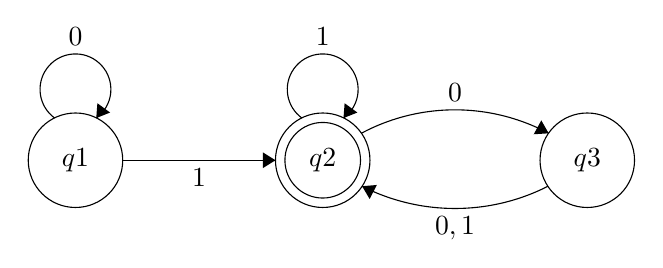
\begin{tikzpicture}[scale=0.2]
        \tikzstyle{every node}+=[inner sep=0pt]
        \draw [black] (16.4,-28.4) circle (3);
        \draw (16.4,-28.4) node {$q1$};
        \draw [black] (32.1,-28.4) circle (3);
        \draw (32.1,-28.4) node {$q2$};
        \draw [black] (32.1,-28.4) circle (2.4);
        \draw [black] (48.9,-28.4) circle (3);
        \draw (48.9,-28.4) node {$q3$};
        \draw [black] (15.077,-25.72) arc (234:-54:2.25);
        \draw (16.4,-21.15) node [above] {$0$};
        \fill [black] (17.72,-25.72) -- (18.6,-25.37) -- (17.79,-24.78);
        \draw [black] (19.4,-28.4) -- (29.1,-28.4);
        \fill [black] (29.1,-28.4) -- (28.3,-27.9) -- (28.3,-28.9);
        \draw (24.25,-28.9) node [below] {$1$};
        \draw [black] (30.777,-25.72) arc (234:-54:2.25);
        \draw (32.1,-21.15) node [above] {$1$};
        \fill [black] (33.42,-25.72) -- (34.3,-25.37) -- (33.49,-24.78);
        \draw [black] (34.554,-26.687) arc (118.10792:61.89208:12.62);
        \fill [black] (46.45,-26.69) -- (45.98,-25.87) -- (45.5,-26.75);
        \draw (40.5,-24.7) node [above] {$0$};
        \draw [black] (46.404,-30.052) arc (-63.08675:-116.91325:13.043);
        \fill [black] (34.6,-30.05) -- (35.08,-30.86) -- (35.54,-29.97);
        \draw (40.5,-31.96) node [below] {$0,1$};
        \end{tikzpicture}
    \end{center}
    \begin{enumerate}
        \item $Q = \left\{q1, q2, q3\right\}$
        \item $\Sigma = \left\{1,0\right\}$
        \item $\delta:Q \times \Sigma \rightarrow Q = ((q1,0),q1), ((q1,1),q2),\ldots$
        \item $F \subseteq Q = \left\{q2\right\}$ 
    \end{enumerate}
\end{frame}

\begin{frame}
    \begin{center}
        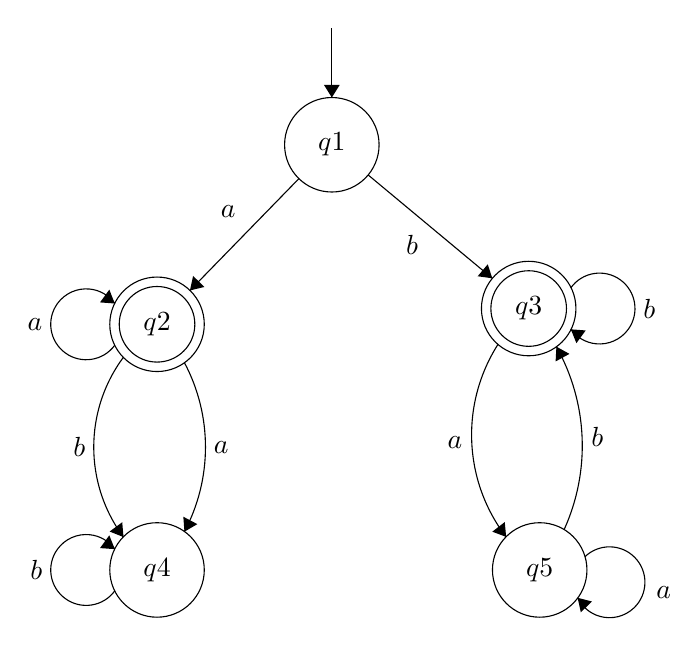
\begin{tikzpicture}[scale=0.2]
        \tikzstyle{every node}+=[inner sep=0pt]
        \draw [black] (36.3,-12.7) circle (3);
        \draw (36.3,-12.7) node {$q1$};
        \draw [black] (25.2,-24.1) circle (3);
        \draw (25.2,-24.1) node {$q2$};
        \draw [black] (25.2,-24.1) circle (2.4);
        \draw [black] (48.8,-23.1) circle (3);
        \draw (48.8,-23.1) node {$q3$};
        \draw [black] (48.8,-23.1) circle (2.4);
        \draw [black] (25.2,-39.7) circle (3);
        \draw (25.2,-39.7) node {$q4$};
        \draw [black] (49.5,-39.7) circle (3);
        \draw (49.5,-39.7) node {$q5$};
        \draw [black] (36.3,-5.3) -- (36.3,-9.7);
        \fill [black] (36.3,-9.7) -- (36.8,-8.9) -- (35.8,-8.9);
        \draw [black] (22.52,-25.423) arc (324:36:2.25);
        \draw (17.95,-24.1) node [left] {$a$};
        \fill [black] (22.52,-22.78) -- (22.17,-21.9) -- (21.58,-22.71);
        \draw [black] (22.52,-41.023) arc (-36:-324:2.25);
        \draw (17.95,-39.7) node [left] {$b$};
        \fill [black] (22.52,-38.38) -- (22.17,-37.5) -- (21.58,-38.31);
        \draw [black] (34.21,-14.85) -- (27.29,-21.95);
        \fill [black] (27.29,-21.95) -- (28.21,-21.73) -- (27.49,-21.03);
        \draw (30.22,-16.93) node [left] {$a$};
        \draw [black] (23.067,-37.608) arc (-143.42715:-216.57285:9.579);
        \fill [black] (23.07,-37.61) -- (22.99,-36.67) -- (22.19,-37.26);
        \draw (20.68,-31.9) node [left] {$b$};
        \draw [black] (26.938,-26.534) arc (28.0065:-28.0065:11.426);
        \fill [black] (26.94,-37.27) -- (27.76,-36.79) -- (26.87,-36.32);
        \draw (28.78,-31.9) node [right] {$a$};
        \draw [black] (38.61,-14.62) -- (46.49,-21.18);
        \fill [black] (46.49,-21.18) -- (46.2,-20.29) -- (45.56,-21.05);
        \draw (41.39,-18.39) node [below] {$b$};
        \draw [black] (51.48,-21.777) arc (144:-144:2.25);
        \draw (56.05,-23.1) node [right] {$b$};
        \fill [black] (51.48,-24.42) -- (51.83,-25.3) -- (52.42,-24.49);
        \draw [black] (47.369,-37.602) arc (-142.60752:-212.56317:10.678);
        \fill [black] (47.37,-37.6) -- (47.28,-36.66) -- (46.49,-37.27);
        \draw (44.62,-31.58) node [left] {$a$};
        \draw [black] (50.559,-25.522) arc (29.29843:-24.46912:12.856);
        \fill [black] (50.56,-25.52) -- (50.51,-26.46) -- (51.39,-25.98);
        \draw (52.75,-31.26) node [right] {$b$};
        \draw [black] (52.369,-38.863) arc (133.99202:-154.00798:2.25);
        \draw (56.87,-41.13) node [right] {$a$};
        \fill [black] (51.91,-41.47) -- (52.11,-42.39) -- (52.82,-41.7);
        \end{tikzpicture}
    \end{center}

    \begin{ejercicio}{}
            Especificar el FA en la figura. Definir el lenguaje.
    \end{ejercicio}
\end{frame}

\begin{frame}
    \begin{center}
        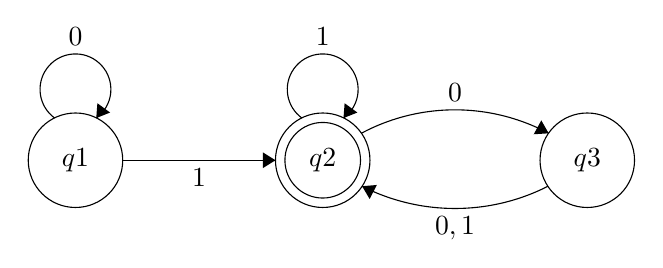
\begin{tikzpicture}[scale=0.2]
        \tikzstyle{every node}+=[inner sep=0pt]
        \draw [black] (16.4,-28.4) circle (3);
        \draw (16.4,-28.4) node {$q1$};
        \draw [black] (32.1,-28.4) circle (3);
        \draw (32.1,-28.4) node {$q2$};
        \draw [black] (32.1,-28.4) circle (2.4);
        \draw [black] (48.9,-28.4) circle (3);
        \draw (48.9,-28.4) node {$q3$};
        \draw [black] (15.077,-25.72) arc (234:-54:2.25);
        \draw (16.4,-21.15) node [above] {$0$};
        \fill [black] (17.72,-25.72) -- (18.6,-25.37) -- (17.79,-24.78);
        \draw [black] (19.4,-28.4) -- (29.1,-28.4);
        \fill [black] (29.1,-28.4) -- (28.3,-27.9) -- (28.3,-28.9);
        \draw (24.25,-28.9) node [below] {$1$};
        \draw [black] (30.777,-25.72) arc (234:-54:2.25);
        \draw (32.1,-21.15) node [above] {$1$};
        \fill [black] (33.42,-25.72) -- (34.3,-25.37) -- (33.49,-24.78);
        \draw [black] (34.554,-26.687) arc (118.10792:61.89208:12.62);
        \fill [black] (46.45,-26.69) -- (45.98,-25.87) -- (45.5,-26.75);
        \draw (40.5,-24.7) node [above] {$0$};
        \draw [black] (46.404,-30.052) arc (-63.08675:-116.91325:13.043);
        \fill [black] (34.6,-30.05) -- (35.08,-30.86) -- (35.54,-29.97);
        \draw (40.5,-31.96) node [below] {$0,1$};
        \end{tikzpicture}
    \end{center}

    \begin{ejercicio}{}
            Especificar el FA en la figura. Definir el lenguaje.
    \end{ejercicio}
\end{frame}

\note{
    Hasta ahora no hablamos de nada mas que el FA. Es decir, el model oque estamos explroando es simple, pero mostramos que 
    puede hacer varias cosas. Puede reconocer letras, puede reconocer patrones, etc. \\
    Tiene poca memoria, como se codifica la memoria? Como piensan que se representa la memoria?
}

\subsection{Definici\'on formal de Computaci\'on. Propiedades de los FA}

\begin{frame}
    \frametitle{Computaci\'on}
    Sea $M = \left(Q,\Sigma, \delta, q_{0}, F\right)$ un FA. Sea $w = w_{1}w_{2}, \ldots, w_{n}$
    una cadena donde $w_{i} \in \Sigma, 0 < i \leq n$. $M$ acepta $w$ si existe una secuencia
    de estados $r_{0},r_{1}, \ldots, r_{m}$  con $r_{i} \in Q, 0 \leq i \leq m $ si:
    \begin{itemize}
        \item $r_{0} = q_{0}$
        \item $\delta(r_{i}, w_{i+1}) = r_{i+1}, 0 \leq i \leq m$
        \item $r_{n} \in F$
    \end{itemize}
    \begin{itemize}
        \item $L\left(M\right)$ es el conjunto de cadenas que acepta $M$.  
        \item $M$ reconoce el lenguaje $A$ si $A = \left\{w | w \in L\left(M\right)\right\}$
    \end{itemize}
    Un lenguaje $A$ es \emph{regular} si existe un FA que lo reconozca.
\end{frame}

\begin{frame}
    \begin{block}{Si yo digo}
        Para contar necesito memoria infinita. ?`Es verdad o mentira?
    \end{block}
    \pause
    \begin{center}
        Es verdad y es mentira.  Depende del modelo. \smiley. 
    \end{center}
\end{frame}

\begin{frame}
    \begin{ejercicio}{}
        Construir un FA que reconozca la siguiente cadena: 111000.\pause
    \end{ejercicio}
    \begin{ejercicio}{}
        Construir un FA que reconozca las siguientes cadenas: $1^n0^n$
    \end{ejercicio}
\end{frame}

\note{
    No se puede! Hacer notar que es la misma cantidad de 1 que de 0. Porque decimos storage infinito>?
    porque si tuvieramos infinitos estados podemos construir todos los posibles combinaciones de iguales. 
}

\begin{frame}
    \frametitle{El pumping lemma}
    Formalmente:
    Si $w \in A$, y $|w| > |Q|$, entonces: \\
    \vspace{2mm}
    $\exists q\in Q~y~x \in \Sigma^{+}$ tal que:
    \begin{enumerate}
        \item $w = yxz$
        \item $\delta^*(q,x) = q$
    \end{enumerate}
    entonces: $yx^nz \in A \forall n \geq 0$\\
    \pause
    Informalmente:\\
    Si existe una cadena en un lenguaje reconocido por un FA que pueda ser descompuesta en tres partes: $y,x,z$ tal que $x$ empiece y termine 
    en el mismo estado, entonces el FA va a reconocer cualquier cadena con un n\'umero arbitrario de $x$.
\end{frame}


\begin{frame}
    \huge{\textcolor{red}{Un FA no puede contar}}
\end{frame}

\note{
    Here we prove it.
    \begin{itemize}
        \item It is not that we say the FA is crap, but rather, an insufficient model. We need to use something more powerful
    \end{itemize}
}

\begin{frame}
    \frametitle{Para hacer en casa}
    \begin{itemize}
        \item Challenge 1 - Números Binarios
        \item Challenge 2 - Demostraci\'on.
    \end{itemize}This 
\end{frame}
